\documentclass[12pt,a4paper]{article}
\usepackage[spanish,es-tabla]{babel}
\usepackage{float}							% Insertar figuras


\usepackage[utf8]{inputenc} % Escribir con acentos, ~n...
\usepackage{eurosym} % s´ımbolo del euro
\newcommand{\horrule}[1]{\rule{\linewidth}{#1}} % Create horizontal rule command with 1 argument of height
\usepackage{listings}             % Incluye el paquete listing
\usepackage{amsfonts}
\usepackage{booktabs}
\usepackage{subfig}

\usepackage[cache=false]{minted}
\usepackage{graphics,graphicx, float} %para incluir imágenes y colocarlas
\usepackage{hyperref}
\hypersetup{
	colorlinks,
	citecolor=black,
	filecolor=black,
	linkcolor=black,
	urlcolor=black
}
\usepackage{multirow}
\usepackage{array}
\usepackage{diagbox}
\usepackage{listings}


\title{
\normalfont \normalsize 
\textsc{{\bf Simulación de Sistemas (2019-2020)} \\ Grado en Ingeniería Informática \\ Universidad de Granada} \\ [25pt] % Your university, school and/or department name(s)
\horrule{0.5pt} \\[0.4cm] % Thin top horizontal rule
\huge Práctica 3 \\ % The assignment title
\horrule{2pt} \\[0.5cm] % Thick bottom horizontal rule

\includegraphics{images/logo.png}	
}

\author{Antonio Jesús Heredia Castillo} % Nombre y apellidos

\date{\normalsize\today} % Incluye la fecha actual

%----------------------------------------------------------------------------------------
% DOCUMENTO
%----------------------------------------------------------------------------------------

\begin{document}

\maketitle % Muestra el Título

\newpage
\tableofcontents % para generar el índice de contenidos
\newpage %inserta un salto de página
\listoffigures
\newpage

\section[Capítulo 1: Mi segundo modelo de simulación discreto]{Capítulo 1\\{\large Mi Segundo Modelo de Simulación Discreto}}
La simulación de este modelo es un problema de cliente-servidor. Primero estudiaremos una simplificación con un solo servidor y varios clientes con un incremento fijo. Sobre esta simulación realizaremos varios experimentos cambiando los datos de entrada tales como los tiempo de llegada, tiempo de servicio y cantidad de clientes que van a llegar. 
\subsection{Simulación con incremento fijo}
A partir del pseudocodigo proporcionado por el profesor hemos creado un modelo de simulación del sistema cliente-servidor donde el incremento usado es fijo. Que el incremento sea fijo no nos impide poder utilizar diferentes unidades de medida. Por ejemplo podemos realizar diferentes experimentos usando incrementos por segundos, minutos, cuartos de hora, etc. \\
Como indica en el enunciado vamos a realizar los distintos experimentos con una cantidad de clientes a atender de 10000 y una cantidad de simulaciones de 150. A partir de estos datos que seran fijos usaremos distintos tiempos de llegada y de servicio. Como indica en el guión de practicas, en caso de que sean horas \textbf{tlleg=0.15} y \textbf{tserv=0.1} . En caso de que quisiéramos hacer medias horas debería ser \textbf{tlleg=0.15x2=0.3} y  \textbf{tserv=0.1x2=0.2} (por que en una hora hay dos medias horas). Así iremos construyendo toda la tabla hasta llegar a décimas de segundo

\begin{table}[H]
	\centering	
	\begin{tabular}{cccccc} \toprule
		{U. Medida}&{tlleg} & {tserv} & {T. Medio} & {Clientes medios} & {T. Ocio} \\ \midrule
		1 hora & 0.15  & 0.1 & 0.00061 & 0.044432 & 0.1326 \\
		1/2 hora & 0.3  & 0.2 & 0.00062 &  0.212586 & 2.92024 \\
		1/4 hora  & 0.6 & 0.4 & 0.00063 & 0.553004 & 11.6528 \\		\midrule
		1 minuto & 9  & 6 & 0.00102 & 1.25661 & 31.5354 \\
		1 segundo  & 540 & 360 & 0.011988 & 1.33738  & 33.3073 \\		\midrule
		1 décima de hora  & 1.5 & 1 & 0.000799 & 0.94829  & 23.0715 \\
		1 décima de minuto  & 90 & 60 & 0.00261484 & 1.31365  & 33.247 \\
		1 décima de segundo  & 5400 & 3600 & 0.11362 & 1.34542  & 33.252 \\ 
		\midrule

	\end{tabular}
	\caption{Simulación Incremento Fijo} \label{tab:iincrementoijo}
\end{table}
Cuanto mas pequeño es el intervalo y por lo tanto los tiempo \textbf{tlleg} y \textbf{tserv} son mayores, los resultados parece que van estabilizándose (o llegando a una cota máxima). Al usar un incremento fijo, cuando usamos valores para \textbf{tlleg} y \textbf{tserv} muy pequeños, al redondear, es muy posible que lo que devuelva sea 0 y por lo tanto tengamos que convertirlo en un 1. Debido a esto iremos acumulando un error en cada una de las generaciones.
\begin{Verbatim*}
	float u = (float) ((float) random()/(RAND_MAX+1.0));
	u = ceil(-tlleg*log(1-u));
	if(u == 0)
		u = 1;
	return u;	
\end{Verbatim*}
El crecimiento tanto del \textbf{T.Medio} y de \textbf{T. Ocio} parece ser que se acerca a una curva logística. El \textbf{Clientes Medios} parece que llega a su máximo entorno a 1.34 y el \textbf{T. Ocio} entorno  al 33.25.\\
Para poder interpretar mejor los resultados vamos a hacer uso de algunas graficas. 
\begin{figure}[H]
	\centering
	\subfloat[Tiempo medio en cola]{
		\label{f:apartadoTiempoMedioCola}
		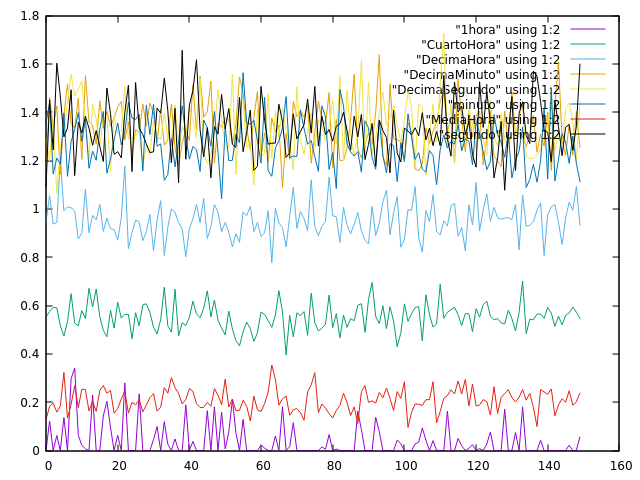
\includegraphics[width=0.5\textwidth]{images/apartado1Col2.png}}
	\subfloat[Porcentaje de Ocio]{
		\label{f:modTablaB}
		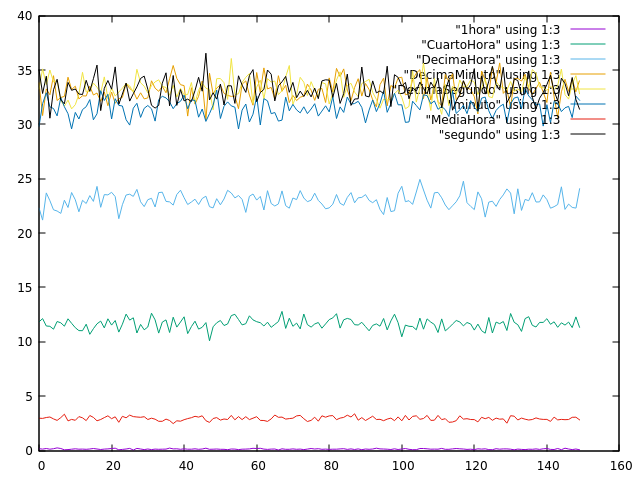
\includegraphics[width=0.5\textwidth]{images/apartado1Col3.png}}
	\caption{Variación de los valores en las distintas simulaciones con incremento fijo.}
	
	\label{f:apartado1_1}
\end{figure}
Como podemos ver mejor aquí, para décima de segundo, décima de minuto y segundo, los valores están todos en el mismo intervalo. En caso de \textbf{T. Ocio} entre 30 y 35. 
\subsection{Simulación con incremento variable}
Ahora el incremento no se realizara en números naturales, en este modelo podremos realizar incremento en números reales evitando así el problema que teníamos a tener que pasar el 0 a 1, por lo tanto al eliminar el error los datos obtenidos deben ser todos mas parecidos entre si. \\
Lo mencionado anteriormente se cumple como podemos ver en la Tabla \ref{tab:iincrementovar}. Con el incremento variable usar distintas unidades de medida no afecta significativamente a los resultados. 
\begin{table}[H]
	\centering	
	\begin{tabular}{cccccc} \toprule
		{U. Medida}&{tlleg} & {tserv} & {T. Medio} & {Clientes medios} & {T. Ocio} \\ \midrule
		1 hora & 0.15  & 0.1 &  0.00109 & 1.34316 &  33.2504 \\
		1/2 hora & 0.3  & 0.2 & 0.00082 &  1.34467 & 33.3121 \\
		1/4 hora  & 0.6 & 0.4 & 0.00092 & 1.33542 & 33.1982 \\		\midrule
		1 minuto & 9  & 6 & 0.00106 & 1.33185 & 33.3748 \\
		1 segundo  & 540 & 360 & 0.00083 & 1.32576  & 33.3792 \\		\midrule
		1 décima de hora  & 1.5 & 1 & 0.00096 & 1.34701  & 33.2438 \\
		1 décima de minuto  & 90 & 60 & 0.00102 & 1.33576  & 33.2355 \\
		1 décima de segundo  & 5400 & 3600 & 0.00091 & 1.33242  & 33.4292 \\ 
		\midrule
		
	\end{tabular}
	\caption{Simulación Incremento Variable} \label{tab:iincrementovar}
\end{table}
Al igual que con el incremento fijo vamos a hacer la comparación usando unas graficas para ver mejor el resultado. A diferencia que en la Figura \ref{f:apartado1_1} en la Figura \ref{f:apartado1_2} podemos ver como tanto el tiempo medio en cola y el porcentaje de tiempo de ocio, se mueven en los mismo intervalos todas las unidades de tiempo. 
\begin{figure}[H]
	\centering
	\subfloat[Tiempo medio en cola]{
		\label{f:apartado1_2Col2}
		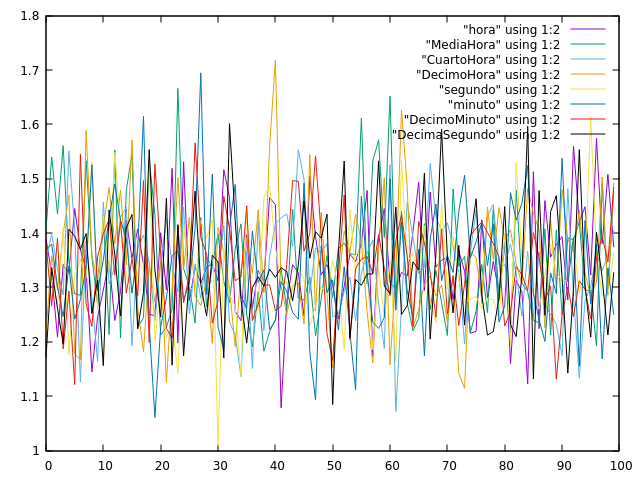
\includegraphics[width=0.5\textwidth]{images/apartado1_2Col2.png}}
	\subfloat[Porcentaje de Ocio]{
		\label{f:apartado1_2Col3}
		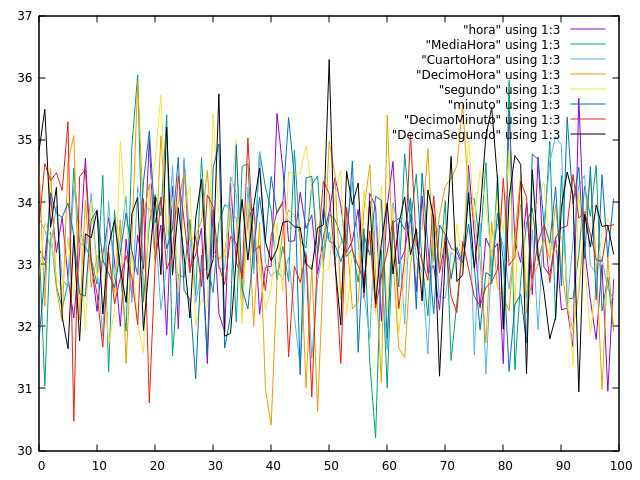
\includegraphics[width=0.5\textwidth]{images/apartado1_2Col3.png}}
	\caption{Variación de los valores en las distintas simulaciones con incremento variable.}
	
	\label{f:apartado1_2}
\end{figure}
Aunque viendo los resultados experimentales podemos ver que el tiempo que esta en ocio, se encuentra entorno al 33.3 y el numero de clientes medios se encuentra en torno al 1.33, veremos si estos resultados concuerdan con los valores que deberíamos obtener de forma teórica. \\
Teniendo en cuenta que cumplimos que $tserv<tlleg$. Primero tenemos que calcular: $\rho=\frac{ tserv }{tlleg }=\frac{6}{9}=0 . \widehat{6}$ y a partir de aquí ya podemos calcular el valor de $Q(n)$ y $PTO(n)$ cuando $n\rightarrow+\infty$.
$$Q(n) = \frac{\rho^2}{1-\rho}=\frac{(\frac{6}{9})^2}{1-\frac{6}{9}}=1.\widehat{3}$$
Como podemos ver, el valor de $Q(n)$ teórico se corresponde con el valor que hemos obtenido con las simulaciones. Ahora pasamos a ver si el valor de $PTO(n)$ corresponde con el teórico.
$$PTO(n)=100*(1-\rho)=100*(1-\frac{6}{9})=100*\frac{3}{9} =33.\widehat{3}$$
En este caso, vuelven a coincidir  el valor teórico con el obtenido a través de los experimentos. Así que podemos dar por validos los resultados de las simulaciones.
\subsection{Simulación con m servidores trabajando en paralelo}
En las secciones anteriores, teníamos un solo servidor. En este caso podemos tener varios servidores pero seguiremos teniendo una sola cola de espera. Para ver que los valores teoricos se siguen cumpliendo (cuando el tiempo tiende a infinito) realizaremos varios experimentos usando $m=1$. Como nos pide en el enunciado del guión, iremos realizando experimentos con tiempos de simulación progresivamente mayores.
\subsubsection{Comprobación de resultados teóricos}
Para poder comprobar que los resultados teóricos concuerdan con los experimentales cuando el tiempo tiende a infinito realizaremos varias simulaciones aumentando el tiempo de simulación pero dejando fijo $tlleg=9$ y $tserv=6$.
 \begin{table}[H]
 	\centering	
 	\begin{tabular}{c|ccccc} \toprule
 		Tiempo de simulación&100 & 1000 & 100000 & 1000000 & 10000000 \\ \midrule
 		\textbf{Tiempo medio espera}   		& 5.15  & 29.535 &  11.924 & 12.479 & 12.112 \\
 		\textbf{Tiempo medio estancia} 		& 11.053  & 35.535 & 17.924 &  18.479 & 18.112 \\
 		\textbf{Media clientes en cola}		& 0.657 & 3.003 & 1.31 & 1.394 & 1.35 \\		\midrule
 		\textbf{Media clientes en sistema} 	& 1.356 & 3.696 & 1.97 & 2.065 & 2.018 \\
 		\textbf{Long media colas no vacias} & 2.119 & 5.844 & 2.997 & 3.096 & 3.019 \\
 		\textbf{\% Tiempo de ocio}  		& 30.076 & 30.631 & 33.981 & 32.845  & 33.147 \\		
 		\textbf{Longitud máxima cola}  		& 3 & 15 & 16 & 34  & 29 \\
 		\midrule		
 	\end{tabular}
 	\caption{Simulación con un solo servidor} \label{tab:colmmk1}
 \end{table}
Ahora comprobaremos con los valores teóricos que deberíamos obtener.
\begin{itemize}
	\item Tiempo medio de espera en cola: $\frac{tserv^2}{tlleg-tserv}=12$
	\item Tiempo medio de estancia en el sistema: $\frac{tserv*tlleg}{tlleg-tserv}=18$
	\item Número medio de clientes en cola: $\frac{tserv^2}{tlleg*(tlleg-tserv)}=1.\widehat{3}$
	\item Número medio de clientes en el sistema: $\frac{tserv}{tlleg-tserv}=2$
	\item Longitud media de colas no vacías: $\frac{tlleg}{tlleg-tserv}=3$
	\item Porcentaje de tiempo de ocio del servidor: $(1-\frac{tserv}{tlleg})*100=33.\widehat{3}$
\end{itemize}
Como podemos ver todos los valores experimentales, con una cantidad de tiempo de simulación los suficiente grande, se acercan mucho a los valores teorices. Así que podemos dar por valido nuestro sistema de simulación. 
\subsubsection{Aumentar el numero de servidores operativos}
Ahora realizaremos experimentos con distinto numero de servidores pero fijando \textbf{tlleg=9} y \textbf{tserv}   al doble del anterior.Es decir si con un servidor tserv=6, con dos servidores tserv=12 y asi sucesivamente Ademas también fijaremos el tiempo de simulación a 1.000.000. Ya que hemos visto en el  experimento anterior, que con esa cantidad de iteraciones llegamos a resultados aproximados a los teóricos. 
 \begin{table}[H]
	\centering	
	\begin{tabular}{c|ccccc} \toprule
		Numero de Servidores&1 & 2 & 4 & 8 & 16 \\ \midrule
		\textbf{Tiempo medio espera}   		& 11.92  & 10.296 &  6.686 & 3.997 & 1.542 \\
		\textbf{Tiempo medio estancia} 		& 17.942  & 22.296 & 30.686 &  51.997 & 97.542 \\
		\textbf{Media clientes en cola}		& 1.325 & 1.51 & 0.745 & 0.446 & 0.171 \\		\midrule
		\textbf{Media clientes en sistema} 	& 1.99 & 2.494 & 3.421 & 5.794 & 10.799 \\
		\textbf{Long media colas no vacias} & 2.988 & 3.150 & 2.929 & 3.020& 3.042 \\
		\textbf{\% Tiempo de ocio}  		& 33.422 & 32.849 & 33.101 & 33.146  & 33.577 \\		
		\textbf{Longitud máxima cola}  		& 24 & 22 & 22 & 23  & 19 \\
		\midrule		
	\end{tabular}
	\caption{Simulación con varios servidores} \label{tab:colmmk1}
\end{table}
Como podemos ver mejor en la Figura \ref{fig:variosservidores} hay varios valores que bajan considerablemente. El tiempo medio de espera y la media de clientes en cola bajan considerablemente. Aunque el tiempo medio de estancia se dispara, esto se debe a que es el tiempo que tarda en ser servido el cliente, pero en esto no podemos reducir tiempo. Si aumentamos el numero de servidores lo que queda claro es que las esperas se reducen aunque el numero de clientes y la frecuencia con la que lleguen sean iguales.
\begin{figure}[ph]
	\centering
	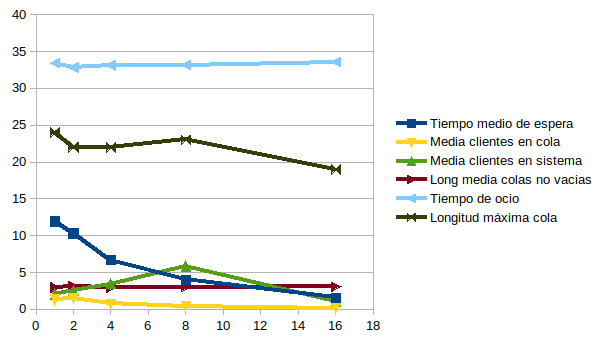
\includegraphics[width=0.7\linewidth]{images/variosservidores}
	\caption{Comparativa de los datos obtenidos usando diferente numero de servidores}
	\label{fig:variosservidores}
\end{figure}
El unico que a priori no cambia es el tiempo en el que el sistema va a estar ocioso. Teniendo así un tiempo en el que el sistema no esta aprovechando su capacidad.
\subsubsection{Modificación media y desviación tipica}
En este punto hemos modificado el código anterior para poder calcular también la desviación típica. La desviación típica nos sirve para ver la dispersión que tiene los datos obtenidos. Cuanto menor sea la desviación típica, mas cercanos estarán los datos a la media. Realizaremos todas las simulaciones con el mismo tiempo de parada, ya que comprobamos anterior mente que con 1.000, los datos obtenidos eran bastante cercanos a los teóricos. Ademas olveremos a realizarlos con un \textbf{tlleg=9} y un \textbf{tserv=6}. Realizaremos pruebas con distinto numero de simulaciones y con un solo servidor siempre para obtener datos cercanos a los teóricos. Para ellos mostraremos dos tablas. Una con los resultados de las medias y otra con el resultado de la desviación típica.\\
En la Tabla \ref{tab:colmmk2} podemos ver las medias:
\begin{table}[H]
	\centering	
	\begin{tabular}{c|ccc} \toprule
		Cantidad de simulaciones&100 & 1000 & 10000   \\ \midrule
		\textbf{Tiempo medio espera}   		& 10.2219  & 10.9616 &  10.7877\\
		\textbf{Tiempo medio estancia} 		& 16.2219  & 16.9616 & 16.7877 \\
		\textbf{Media clientes en cola}		& 1.16 & 1.2568 & 1.2353\\		\midrule
		\textbf{Media clientes en sistema} 	& 1.81 & 1.9175 & 1.889 \\
		\textbf{Long media colas no vacias} & 2.6363 & 2.708 & 2.689 \\
		\textbf{\% Tiempo de ocio}  		& 35.2797 & 33.9292 & 34.636 \\		
		\textbf{Longitud máxima cola}  		& 7.28 & 7.511 & 7.412 \\
		\midrule		
	\end{tabular}
	\caption{Medias en distinta cantidad de simulaciones} \label{tab:colmmk2}
\end{table}
En la Tabla \ref{tab:colmmk2_2} podemos ver la desviación típica:
\begin{table}[H]
	\centering	
	\begin{tabular}{c|ccc} \toprule
		Cantidad de simulaciones&100 & 1000 & 10000  \\ \midrule
		\textbf{Tiempo medio espera}   		& 5.31  & 6.2826 &  6.5803\\
		\textbf{Tiempo medio estancia} 		& 5.31  & 6.2826 & 6.5803 \\
		\textbf{Media clientes en cola}		& 0.6641 & 0.7955 & 0.8337 \\		\midrule
		\textbf{Media clientes en sistema} 	& 0.7218 & 0.862 & 0.8976   \\
		\textbf{Long media colas no vacias} & 0.9094 & 1.023 & 1.062  \\
		\textbf{\% Tiempo de ocio}  		& 7.48678 & 8.7020 & 8.4878   \\		
		\textbf{Longitud máxima cola}  		& 2.59 & 2.77 & 2.79 \\
		\midrule		
	\end{tabular}
	\caption{Desviación típica en las distintas simulaciones} \label{tab:colmmk2_2}
\end{table}
Como podemos ver en las tablas anteriores no afecta el numero de simulaciones para los resultados de estas estadísticas. Todos se mueven en valores muy similares.
\subsubsection{Uso de distintos generadores de datos}
En el guión de la practica nos pide que remplacemos el generador exponencial por generadores determinísticos  que siempre devuelve los valores medios y por generadores uniformes(con la misma media que los anteriores). \\A continuación podemos ver una tabla comparando los tres generadores de datos. En los tres hemos usado un\textbf{tlleg=9} y un \textbf{tserv=6}.

\begin{table}[H]
	\centering	
	\begin{tabular}{c|ccc} \toprule
		Tipo de generador&Uniforme & Exponencial & Determinístico  \\ \midrule
		\textbf{Tiempo medio espera}   		& 11.184  & 0 &  5\\
		\textbf{Tiempo medio estancia} 		& 17.184  & 6 & 11.217 \\
		\textbf{Media clientes en cola}		& 1.2895 & 0 & 0.605 \\		\midrule
		\textbf{Media clientes en sistema} 	& 1.9420 & 0.661 & 1.205   \\
		\textbf{Long media colas no vacias} & 2.82385 & -nan & 2.478  \\
		\textbf{\% Tiempo de ocio}  		& 34.7448 & 33.9 & 39.97   \\		
		\textbf{Longitud máxima cola}  		& 7.73 & 0 & 7 \\
		\midrule		
	\end{tabular}
	\caption{Desviación típica en las distintas simulaciones} \label{tab:colmmk2_2}
\end{table}

Viendo los resultados teóricos obtenidos en los puntos anteriores, podemos ver que el que mejor se ajusta a este problema, sigue siendo el exponencial.
\section[Capítulo 2: Mi tercer modelo de simulación discreto]{Capítulo 2\\{\large Mi Tercer Modelo de Simulación Discreto}}
En este modelo vamos a simular un puerto de carga. El puerto tiene capacidad para operar con 3 petroleros a la vez. Los petroleros llegan cada $11\pm7$ horas. Ademas existen tres tipos de barcos y estos llegan con una frecuencia relativa  y tienen un tiempo de carga distinto.
\begin{table}[h]
	\centering
	\begin{tabular}{c|cc}\toprule
		Tipo&Frec.Relativa&Tiempo de carga(horas)\\\midrule
		1&0.25&$18\pm2$\\
		2&0.25&$24\pm3$\\
		2&0.5&$36\pm4$\\
	\end{tabular}
\end{table}
Para mas detalles ver el guión de la practica.
\subsubsection{Probando el modelo}
Lo primero que vamos a realizar es ver como funciona el modelo sin añadir ninguna modificación. De esta forma obtendremos unos datos desde los cuales partir. Para ver el funcionamiento del modelo realizaremos varias simulaciones cambiando el numero de simulaciones que se realiza. Como es de esperar, cuantas mas simulaciones datos mas "estabilizados" obtendremos. Esto es interesante para ver con que cantidad nos quedamos de cara a las siguientes simulaciones.
\begin{table}[h]
	\centering
	\begin{tabular}{c|cccc}\toprule
		Numero simulaciones&10&100&1000&10000\\\midrule
		Media Barco en cola de llegada&1.2583&1.2106&1.2079&1.2183\\
		Media Barco en cola de salidas&0.0262&0.0286&0.0288&0.0288\\
		T estancia en puerto (tipo 0)&34.098&33.7427&33.6633&33.7809\\
		T estancia en puerto (tipo 1)&40.034&39.5465&39.6256&39.7218\\
		T estancia en puerto (tipo 2)&52.139&51.5185&51.50444&51.6068\\
		\% tiempo remolcador desocupado&80.6813&80.6313&80.6335&80.625298\\
		\% tiempo remolcador viajando vacio&1.2542&1.2382&1.2662&1.2625\\
		\% tiempo remolcador remolcando&18.064&18.1304&18.1001&18.1120\\
		\% tiempo atraques libres&13.093&12.9832&13.0324&13.0276\\
		\% tiempo atraques ocupados sin cargar&0.873&0.9526&0.962&0.9603\\
		\% tiempo atraques ocupados cargando&86.0332&86.064&86.0073&86.0121\\
	\end{tabular}
	\caption{Resultados del modelo sin modificar} \label{tab:petrolero_1}
\end{table}
Como podemos ver en la Tabla \ref{tab:petrolero_1}, no nos merece la pena aumentar el numero de simulaciones mucho. Esto se puede ver ya que la diferencia entre realizar 100,1000 o 10000 es mínima. Por lo tanto nos quedaremos con un numero de simulaciones de 100. \\
Como podemos ver, la mayoría del tiempo los atraques están ocupados cargando y que el tiempo que permanecen en el atraque  sin estar realizando operación de carga, es bastante pequeño. A priori parecería interesante aumentar el numero de atraques del puerto, sin ser necesario otro remolcador, ya que la mayoría del tiempo esta desocupado.
\subsubsection{Aumento del numero de atraques}
En el guión de la practica nos pide que realicemos distintas modificaciones al modelo original. Una de ellas es que aumentemos el numero de atraques disponibles. Aunque lo que yo he realizado es generar un modelo que te deje usar la cantidad de atraques que queramos, las pruebas que vamos a realizar es solo de tres(el anterior), cuatro y cinco atraques disponibles. Para solo tres atraques disponibles usaremos los datos anteriores con el numero de simulaciones de 100.
\begin{table}[h]
	\centering
	\begin{tabular}{c|ccc}\toprule
		Numero de atraques&3&4&5\\\midrule
		Media Barco en cola de llegada3&1.2106&0.0415&0.006\\
		Media Barco en cola de salidas&0.0286&0.0080&0.007\\
		T estancia en puerto (tipo 0)&33.7427&20.5242&20.1669\\
		T estancia en puerto (tipo 1)&39.5465&26.5727&26.1619\\
		T estancia en puerto (tipo 2)&51.5185&38.5294&38.1569\\
		\% tiempo remolcador desocupado&80.6313&81.8771&81.8818\\
		\% tiempo remolcador viajando vacio&1.2382&3.6275&3.9888\\
		\% tiempo remolcador remolcando&18.1304&18.1228&18.1181\\
		\% tiempo atraques libres&12.9832&35.224&48.1852\\
		\% tiempo atraques ocupados sin cargar&0.9526&0.19999&0.537\\
		\% tiempo atraques ocupados cargando&86.064&64.5755&51.6610\\
	\end{tabular}
	\caption{Resultados del modelo con distintos atraques disponibles} \label{tab:petrolero_2}
\end{table}
Como podemos ver en la Tabla \ref{tab:petrolero_2} aumentar el numero de atraques disponibles no afecta mucho  a las estadísticas que afectan al remolcador. Por ejemplo el porcentaje de tiempo que el remolcador da viajes vacíos ha aumentado. Esto de puede deber al hecho de que tenga que ir a por barcos sin tener que sacar ninguno del puerto.\\\\
Donde mas se ha notado la mejora ha sido en el tiempo en que los barcos están en el puerto, disminuyendo dastricamente. También ha mejorado el tiempo en que los atraques están ocupados cargando, pero esto se puede deber a que no siempre hay barcos para ocupar todos los atraques.\\\\
Viendo los datos y si fuera el caso de que el puerto nos pidiera recomendación de aumentar el puerto en un o dos atraques, le recomendaría que solo aumentara en uno. Ya que posiblemente el coste de ampliar mas no merecería la pena.

\subsubsection{Cambiar el remolcador por uno al que no le afecta las tormentas}
Como en el caso anterior realizaremos la comparación con los datos de la Tabla \ref{tab:petrolero_1} con un numero de simulaciones de 100.
\begin{table}[h]
	\centering
	\begin{tabular}{c|cc}\toprule
		Afectan las tormentas&SI&NO\\\midrule
		Media Barco en cola de llegada3&1.2106&1.06\\
		Media Barco en cola de salidas&0.0286&0.0278\\
		T estancia en puerto (tipo 0)&33.7427&32.1712\\
		T estancia en puerto (tipo 1)&39.5465&37.771\\
		T estancia en puerto (tipo 2)&51.5185&49.9415\\
		\% tiempo remolcador desocupado&80.6313&81.9218\\
		\% tiempo remolcador viajando vacío&1.2382&1.612\\
		\% tiempo remolcador remolcando&18.1304&18.07\\
		\% tiempo atraques libres&12.9832&13.2928\\
		\% tiempo atraques ocupados sin cargar&0.9526&0.9283\\
		\% tiempo atraques ocupados cargando&86.064&85.7787\\
	\end{tabular}
	\caption{Resultados del con remolcador al que le afecta las tormentas y otro al que no} \label{tab:petrolero_3}
\end{table}
Viendo los datos obtenido en la Tabla \ref{tab:petrolero_3} parece ser que no hay mucha diferencia entre usar un petrolero al que le afecte las tormentas y otro al que no. No hay cambios significativos en el modelo, esto se puede deber a que la probabilidad de tormenta sea bastante baja.
\subsubsection{Cambiar el remolcador por uno mas rápido}
Como en el caso anterior realizaremos la comparación con los datos de la Tabla \ref{tab:petrolero_1} con un numero de simulaciones de 100.
\begin{table}[H]
	\centering
	\begin{tabular}{c|cc}\toprule
		Velocidad&0.25&0.15\\\midrule
		Media Barco en cola de llegada3&1.2106&1.2636\\
		Media Barco en cola de salidas&0.0286&0.0283\\
		T estancia en puerto (tipo 0)&33.7427&34.2127\\
		T estancia en puerto (tipo 1)&39.5465&40.092\\
		T estancia en puerto (tipo 2)&51.5185&52.093\\
		\% tiempo remolcador desocupado&80.6313&81.13\\
		\% tiempo remolcador viajando vacío&1.2382&0.07158\\
		\% tiempo remolcador remolcando&18.1304&18.1516\\
		\% tiempo atraques libres&12.9832&12.7852\\
		\% tiempo atraques ocupados sin cargar&0.9526&0.94412\\
		\% tiempo atraques ocupados cargando&86.064&86.2706\\
	\end{tabular}
	\caption{Resultados del modelo con distintas velocidades de movimiento vacío} \label{tab:petrolero_4}
\end{table}
En este caso, como era de esperar, el tiempo que mas a mejorado es el porcentaje de viaje en vacío que ha bajado de 1. El barco, al ser mas rápido tarda menos tiempo en salir del puerto a coger un nuevo barco.
\end{document}
	